\documentclass[10pt]{article}

\usepackage[margin=0.85in]{geometry}
\usepackage{booktabs}
\usepackage{graphicx}
\usepackage{hyperref}
\usepackage{enumitem}
\graphicspath{{../slides/assets/figures/}}

\title{Test-Time Physical Awareness for Generated Humanoid Reference Motions}
\author{Tae Hoon Yang\\CS 348K: Visual Computing Systems}
\date{Spring 2026}

\begin{document}
\maketitle

\begin{abstract}
Modern humanoid motion trackers such as SONIC can follow rich whole-body
reference trajectories in physics, but those trackers still need high-quality
reference motions. KIMODO makes reference authoring much easier by generating
Unitree G1 kinematic motions from text prompts and constraints. This project
studies the interface between those systems: given a generated G1 reference,
can we detect physical risks, use those risks to rewrite the prompt, regenerate
better candidates, and then gate the result with a controller rollout?

I built a test-time physical-awareness loop. It evaluates generated references
with MuJoCo inverse-dynamics/contact diagnostics and a pretrained SONIC
controller audit. The evaluator emits interpretable failure tags such as high
torque/root wrench, self-contact, non-foot floor contact, weak support, contact
artifact, and controller trackability failure. Those tags are passed as
structured context to GPT-5.5, which rewrites the prompt with a metric-specific
safety constraint. On the 100-prompt KIMODO benchmark, first-pass references
pass the physical screen in 48/100 cases, complete the 4-second SONIC rollout
in 53/100 cases, and pass both gates in 29/100 cases. The final deck reports a
prompt-repair snapshot where metric-guided rewriting reduces several failure
tags, including SONIC fall cases from 47 to 20. The contribution is not a
solved text-to-robot motion generator; it is a concrete evaluation,
prompt-repair, and acceptance gate for exposing generated-reference brittleness.
\end{abstract}

\section{Problem}

Humanoid motion control has recently improved because learned policies can be
trained to track diverse reference motions under physics. SONIC is a strong
example: it trains a Unitree G1 whole-body controller on over 100M frames / 700
hours of high-quality human motion \cite{sonic}. At the input level, the
tracker receives a target trajectory: root pose and joint targets over time.

The upstream question is where those references come from. KIMODO generates
controllable kinematic human and robot motions from text prompts and
constraints \cite{kimodo}. This makes it a natural source of candidate
references for robot training and controller testing. However, a kinematic
reference is not automatically physically executable. It may demand unrealistic
torques, require impossible support, create self-collisions, drag contacts, or
destabilize a learned controller.

The project question is:
\begin{quote}
Can a physical-awareness layer identify risky KIMODO-generated humanoid
reference motions, and can its failure tags guide useful test-time prompt repair
before controller execution?
\end{quote}

\section{System}

The final system is a prompt-refinement loop:

\begin{center}
\begin{tabular}{llll}
\toprule
Stage & Input & Contribution & Output \\
\midrule
Generate & text prompt & KIMODO G1 generation & root + joint trajectory \\
Evaluate & reference & MuJoCo + SONIC checks & risk flags and rollout metrics \\
Rewrite & failed metric tag & GPT-5.5 prompt edit & revised prompt \\
Repeat/gate & new candidate & rescore until budget ends & accepted or flagged clip \\
\bottomrule
\end{tabular}
\end{center}

Failure tags are intentionally interpretable. High torque/root wrench asks the
LLM for slower, smoother limb motion; self-contact asks for limbs away from the
torso; weak support asks for wider stance; trackability failure asks for lower
speed and amplitude. SONIC is used as a foundation-style tracking evaluator and
acceptance gate. It is not the optimizer that edits KIMODO.

\section{Benchmark and Metrics}

The benchmark contains 100 humanoid robotics prompts grouped as locomotion and
recovery (26), manipulation and loco-manipulation (26), floor/low posture (12),
dance/expressive motion (12), athletic and terrain stress (16), and
communication/safety gestures (8). The suite includes walking, shuffling,
crawling, carrying, panel pressing, gestures, obstacle-style steps, forward
rolls, cartwheel attempts, jumping, and low-posture motions.

For each generated G1 trajectory, the evaluator computes torque demand relative
to actuator limits, root force/torque, velocity, acceleration, jerk,
self-contact, non-foot floor contact, contact artifacts, support-region proxy
violations, SONIC no-fall, survival time, and joint RMSE.

\section{Results}

\subsection{First-Pass Audit}

\begin{table}[h]
\centering
\caption{First-pass 100-prompt KIMODO audit.}
\label{tab:audit}
\begin{tabular}{lrrrrr}
\toprule
Set & Physical pass & SONIC no-fall & Both & Mean sec. & RMSE \\
\midrule
All KIMODO refs & 48/100 & 53/100 & 29/100 & 2.855 & 0.156 \\
Physical-pass subset & 48/48 & 29/48 & 29/48 & 3.293 & 0.170 \\
Flagged subset & 0/52 & 24/52 & 0/52 & 2.450 & 0.143 \\
\bottomrule
\end{tabular}
\end{table}

\begin{figure}[h]
\centering
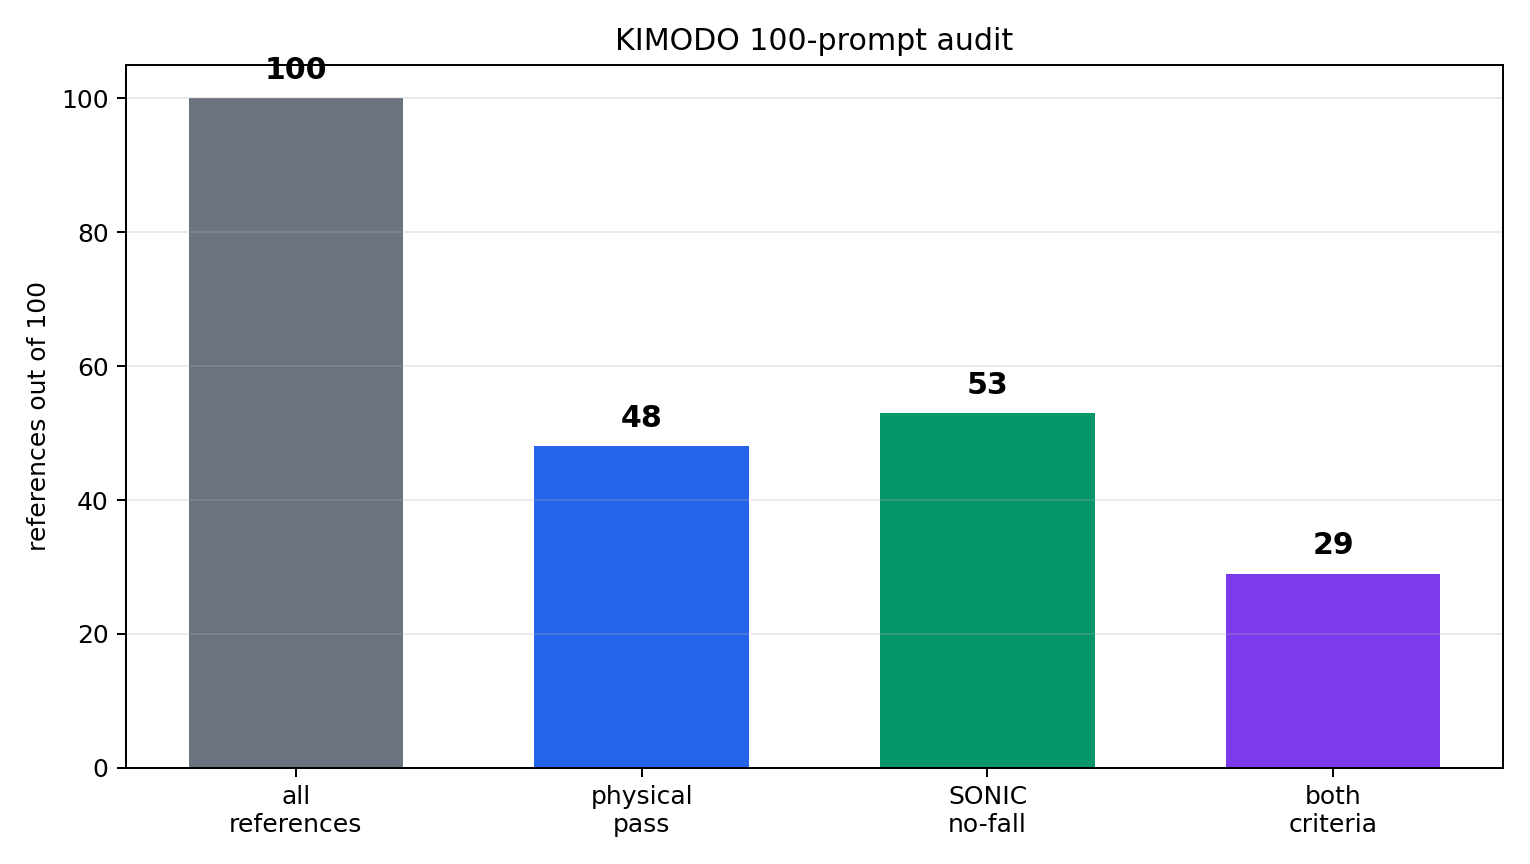
\includegraphics[width=0.82\linewidth]{kimodo_audit_summary.png}
\caption{The physical screen and SONIC audit are related but not equivalent.}
\end{figure}

Only 29 of 48 physical-pass references also complete SONIC. Meanwhile, 24 of
52 flagged references still complete SONIC. This disagreement is a central
result: reference-level physical checks and controller-level trackability are
both needed.

\subsection{Failure Tags}

\begin{table}[h]
\centering
\caption{Failure-tag counts before and after metric-guided prompt repair. Tags
are non-exclusive.}
\label{tab:repairtags}
\begin{tabular}{lrr}
\toprule
Failure tag & Before & After \\
\midrule
SONIC fall & 47 & 20 \\
Torque limit $>$1x & 48 & 23 \\
Self-contact $>$8\% & 34 & 10 \\
Unstable center of mass & 31 & 20 \\
High root force $>$5 kN & 28 & 9 \\
Non-foot floor contact & 11 & 4 \\
\bottomrule
\end{tabular}
\end{table}

The representative failure videos in the deck are `forward\_roll' for
torque/root wrench, `turn\_in\_place' for self-contact, `knee\_slide' for
non-foot floor contact, `step\_over\_right' for support proxy, `carry\_box' for
controller trackability, and `happy\_dance' for contact artifact.

\subsection{Repair Examples}

The main repair videos show failure-tag-guided prompt edits:
`forward\_walk' becomes slower and smoother after a trackability flag;
`wave' adds planted feet and smooth arm motion after torque/tracking flags;
`split\_squat\_jump' asks for a smaller jump and soft landing after
support/torque flags; `pushup\_pose' asks for lifted torso clearance;
`happy\_dance' asks for clean foot placement; and `backward\_recovery' asks for
a smaller lean and step back.

\section{Interpretation}

The results support the hypothesis in a bounded way. Generated references have
measurable physical failure modes; failure tags are useful for prompt
refinement and curation; SONIC is stricter than kinematic replay; and
visual/VLM review helps catch obvious behavior mismatch, but it is not a
complete metric set.

The boundary slide shows remaining failures: `forward\_roll' for torque/root
wrench stress, `carry\_box' for controller trackability, and
`cartwheel\_attempt' for acrobatics. The current method does not solve arbitrary
text-to-robot motion, robust acrobatics/low-posture tracking, or automatic
repair for every invalid reference. Stronger results likely require fine-tuning
or training a motion-level refiner, not only prompt rewriting.

\section{Limitations and Future Work}

GPT-5.5 prompt repair is useful but cannot replace a better motion generator.
The physical screen is heuristic and simulator-dependent. SONIC rollout is a
simulation diagnostic, not real hardware validation. Some motions need semantic
context: floor contact can be correct for crawling and wrong for walking.
Prompt fidelity is checked qualitatively; there is no full human-study or VLM
benchmark.

Future work should train a risk-conditioned refiner that learns from failure
tags and SONIC rollouts, use short controller rollouts or a learned surrogate
during candidate selection, and improve semantic evaluation so physical
stability does not hide prompt mismatch.

\section{Team Responsibilities}

Tae Hoon Yang completed the project solo: prompt suite design, KIMODO/SONIC
integration, MuJoCo physical checks, prompt-repair loop, video rendering, slide
deck, and final report.

\bibliographystyle{plain}
\bibliography{references}

\end{document}
